\documentclass{aastex6}
\usepackage{siunitx}
\usepackage{wrapfig, lipsum, booktabs}
\usepackage{graphicx}
\usepackage{multirow}

\begin{document}
\title{CCD Laboratory Write-up}
\author{B. Connor McClellan, Julieanna Bacon, John Michael Della Costa}
\affil{University of Florida}
\email{cmcclellan1010@ufl.edu}
\and


\begin{abstract}
This lab report outlines the procedures and results of analyzing dark-frame and flat-frame images on a CCD to experimentally measure read noise, dark current, gain, and linearity. I reduce my data in Python 2.7. The objective of the lab is to understand the basic operating principles of a CCD. A large component of this experiment and the following analysis focuses on quantifying error. It is crucial to understand the misgivings of the instrument one is working with before pointing it at actual targets; then, not only can one optimally configure the instrument to acquire the best data possible, but also its error will be well-defined and easily corrected for.
\end{abstract}


\section{EXPERIMENT SETUP}
    Our setup consists of a "dark room" made from two large wooden platforms standing on end, with a heavy, opaque cloth laid on top. At the far end, a piece of flat white paper is suspended vertically on a metal mount. The SBIG CCD, fitted with a Nikon AF NIKKOR 70-300mm lens with a 3-D printed adapter, sits in the middle of the rig with the field of view centered on and perpendicular to the sheet of paper. A large laptop is placed at the opposite end, with the screen casting light from just above the CCD toward the sheet of paper. When we take data, the opaque cloth is set over the entire rig and remains in the same place for the duration of imaging, to preserve consistency in what small amount of light manages to leak through from the outside environment. A small flap on one side is lifted to access the camera, cover the lens, and alter the laptop screen brightness as needed for the experiment. A second laptop is wired to the CCD, and operated from outside the cloth. This laptop, running CCDOps, controls the exposure time, number of images acquired, filters used, and type of exposure.


\section{MEASURING THE READ NOISE}

\subsection{Objective}
    In this section, I quantify the read noise of the detector using 18 0.1-second dark exposures. I then use the same method to find the read noise for increasing exposure times, using 6 1s images, 6 10s images, and 3 100s images.The overall goal of this section is to, first, measure the read noise of the detector accurately, and second, prove that exposure time has no effect on the read noise of the detector. Since read noise is only introduced when the CCD is read out, it only happens once per exposure and should be constant no matter how long the exposure is. To prove this, a linear fit of the read noises at each exposure time should have no appreciable slope; that is, there should be very little correlation between exposure time and read noise.

\subsection{Method}
    I start by loading in the 18 0.1-second images into a 3-dimensional numpy array. Two of the axes are the dimensions of the image, and the third axis is the dimension along which the 18 images are stacked. I then calculate the RMS of the 3-dimensional array along the third axis, using

\begin{equation}
    RMS = \sqrt{|\langle x^2 \rangle-\langle x \rangle^2|}\label{eq:1}
\end{equation}

    This returns a new 2-dimensional array containing the RMS of each pixel in that pixel's location. As stated in the lab manual, the median or mean of this array should be the average read noise of the CCD. The associated uncertainty is

\begin{equation}
    RMSE = \frac{\sigma}{\sqrt{n_{pix}}}\label{eq:2}
\end{equation}

    where $ \sigma $ is the RMS of the array and $ n_{pix} $ is the number of pixels in the CCD. For any set of images in this lab, I will use this definition to calculate the uncertainty of the average of those images.
\par
    An alternate method of measuring the read noise involves plotting the data number (DN) of all the pixels on a histogram, and fitting a Gaussian to the histogram (REFERENCE FIGURE). The central peak of the histogram returns the average read noise of the CCD, and the Gaussian fit's $ \sigma $ describes the statistical spread, which can then be converted to an uncertainty using equation \ref{eq:2}.

\subsection{Results}

\subsubsection{Quantification of Read Noise}

\begin{wraptable}{l}{6.5cm}
    \caption{Read Noise, in DN}
    \label{wrap-tab:1}
    \begin{tabular}{l | c | c}
        \toprule
        Measurement & Average & Gaussian Fit \\
        \midrule
        Mean        & 11.832  & 11.497  \\
        Median      & 11.605  & - \\
        RMS         & 2.512   & 2.424 \\
        RMSE        & \num{4.02e-3} & \num{3.88e-3}\\
        \bottomrule
    \end{tabular}
\end{wraptable}

    The values under "Average" in Table~\ref{wrap-tab:1} are acquired using np.mean, np.median, and my function for calculating RMS and RMSE (RMS Error). They represent the mean, median, and RMS of the stacked data from the 18 0.1-second exposures. The values under "Gaussian Fit" are the returned parameters of the Gaussian fit of the distribution, with $ RMS = \sigma $ of the curve, and $ RMSE = \frac{\sigma}{\sqrt{n_{pix}}} $ . They are indeed similar, though the Gaussian Fit values are smaller across the board. Since the distribution of DNs for these images is not Gaussian, but in fact Poisson, the fit looks noticeably skewed (see Figure \ref{fig:1}). The Gaussian lies just right of the true peak of the histogram, but what really throws the measure of central tendency off is the bins on the right-hand side of the histogram. The bin values are higher on the right side of the peak than the left, so both the raw mean and median calculations get thrown off by the unequal weight. The gaussian, which is roughly centered at the histogram's peak, does not suffer the same fate, and as such has a lower mean and $ \sigma $.

\centering
    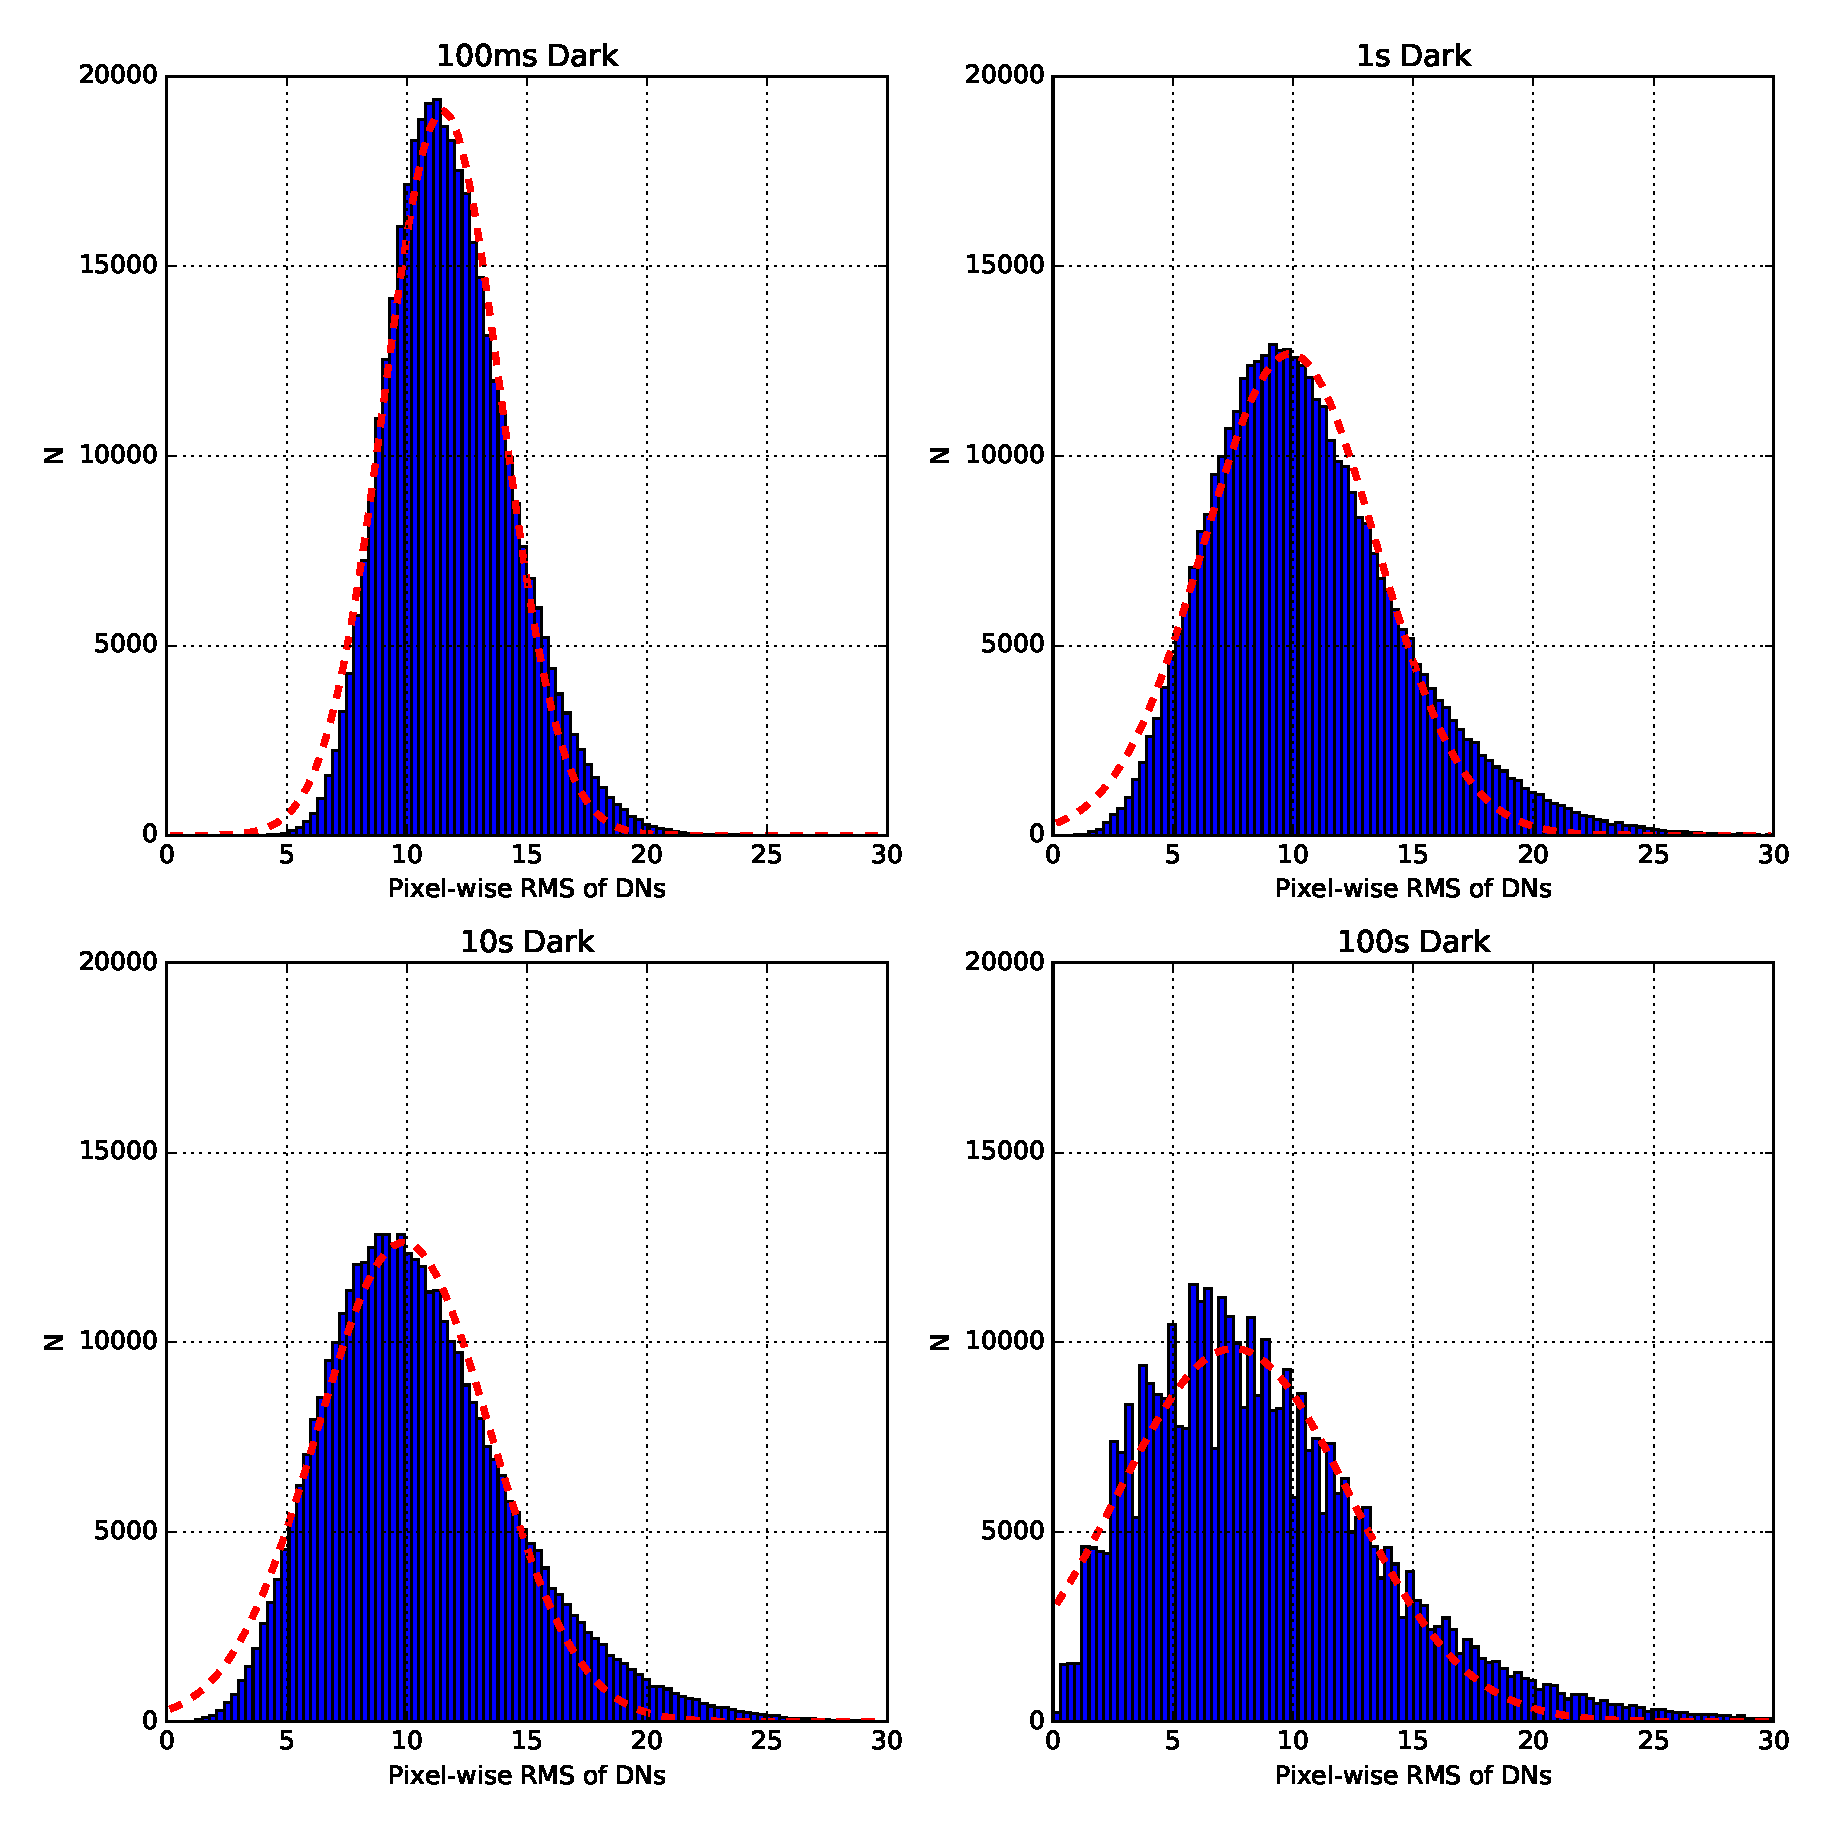
\includegraphics[scale=0.5]{readnoise_histograms}
    \caption{\label{fig:rn_hist} Read Noise Histograms and Gaussian Fits}

\subsubsection{Read Noise Dependence on Time}

\begin{table}
    \caption{Read Noise, in DN}
    \begin{tabular}{c c c c c c c c c}
        \toprule
        \multirow{2}{*}{Measurement}
            & \multicolumn{2}{c}{0.1 s}
                & \multicolumn{2}{c}{1 s}
                    & \multicolumn{2}{c}{10 s}
                        &\multicolumn{2}{c}{100 s} \\
        \cmidrule{2-9}
        & Average & Gaussian & Average & Gaussian & Average & Gaussian & Average & Gaussian \\
        \midrule
        $ Mean $ & 11.832 & 11.497 & 10.650 & 9.871 & 10.657 & 9.874 & 8.982 & 7.512 \\
        $ RMS $ & 2.512 & 2.424 & 3.996 & 3.587 & 4.008 & 3.606 & 5.618 & 4.848 \\
        $ RMSE $ & \num{4.021e-3} & \num{3.881e-3} & \num{6.397e-3} & \num{5.743e-3} & \num{6.417e-3} & \num{5.773e-3} & \num{8.995e-3} & \num{7.761e-3} \\
        \bottomrule
    \end{tabular}
\end{table}


    Read noise is not a function of exposure time. Plotting the peaks of the Gaussian fits in the previous section against their corresponding exposure times yields a linear fit with a slope close to 0. This is expected, since the read noise should not increase or decrease appreciably as exposure time increases. This is shown graphically in Figure \ref{fig:rn_time}, in which the fit has a slope of order $ 10^{-2} $ and the data points themselves don't seem to have any sort of trend. In fact, the only trend the linear fit was able to extract is that read noise actually \texit{decreases} slightly with time, which doesn't make much physical sense. Read noise is not a function of time, since the read noise doesn't increase or decrease as exposure time increases. This confirms the answer to another question: is there a light leak in the camera? If light was leaking into the CCD, though the shutter was closed and the lens cap was on, then the CCD would be collecting photons as the exposure was being taken. The longer the exposure, the more photons the CCD would collect. Thus, with a light leak, longer dark frames would have higher counts per pixel than shorter ones, and the fitted line in Figure \ref{fig:rn_time} would have a positive slope (increasing DN with time). Since this is not the case, I'm pleased to report there is not a light leak in our setup.

\subsection{Summary}

    Examination of the visual data in this section deftly confirms the theory behind read noise. Noise generated by a predictable, one-time electronic procedure should be consistent each time the CCD is read out, and, judging by the results of this section of the lab, it is. Two different statistical methods yield highly similar results for the mean, RMS, and RMSE of the DNs for each of 4 exposure times. This shows that read noise can be approximated as either the mean or peak of a gaussian fit of the pixel-wise RMS of a dark frame, with reasonable accuracy.

\end{document}


\section{MEASURING DARK CURRENT}

\subsection{Objective}
    I measure dark current of the detector by taking a series of longer and longer dark exposures, subtracting the bias from each, and calculating the change in DN with time ( $ \frac{dDN}{dt} $ ). The purpose of measuring the dark current is to find how many thermally-generated electrons accumulate in the CCD before it is read out. It can be mitigated by effective cooling, but not eliminated entirely, and therefore it's important to be able to measure its impact on one's images.

\subsection{Method}
    I begin by measuring my baseline, taking a 0.1-second dark exposure. I then increase the exposure time by a factor of 5, taking one image per exposure time. The exposure times I collected were 1s, 5s, 25s, 125s, and 600s. This is a wide enough range to ensure that even small slopes are noticeable, and not due to error. A bias image is taken every other exposure in order to ensure that the offset doesn't drift. As a precaution, I examined the bias level inbetween each image. The average bias is consistent at 982 DN, with an RMS of 18.7, for all 5 bias images. A median-combined master bias is created from these 5 images, and subtracted from the longer exposures. Now, I'm working with just the dark current.
\subsection{Results}
\subsection{Summary}
